% Standalone compile target for the architecture figure.
% Compile with: pdflatex fig_architecture_standalone.tex
% Produces fig_architecture_standalone.pdf (native vector, grayscale-safe).
% This is the SAME tikzpicture body embedded directly in stbv_paper.tex's
% Fig.~\ref{fig_architecture} -- kept in sync manually; if one changes, so
% should the other.
\documentclass[tikz,border=4pt]{standalone}
\usepackage{tikz}
\usetikzlibrary{arrows.meta,positioning,fit,backgrounds}
\begin{document}
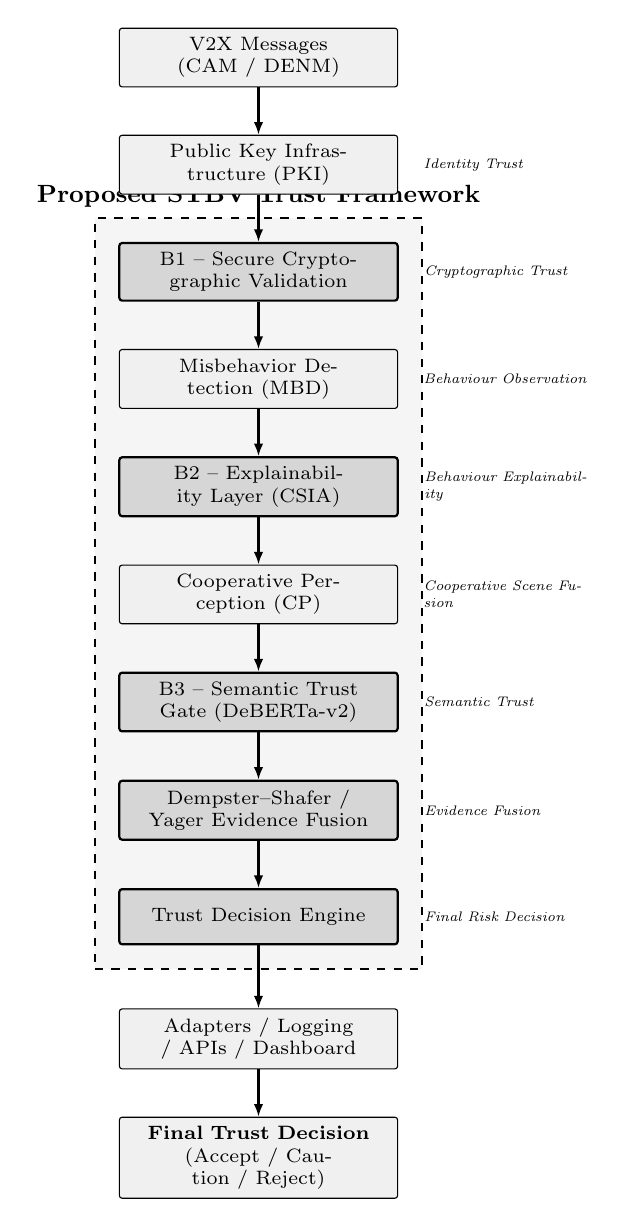
\begin{tikzpicture}[
  font=\scriptsize,
  node distance=6mm and 4mm,
  box/.style={draw, rectangle, rounded corners=1pt, minimum width=3.5cm,
    minimum height=7mm, align=center, text width=3.3cm},
  existing/.style={box, fill=black!6},
  proposed/.style={box, fill=black!16, thick},
  lbl/.style={font=\tiny\itshape, text width=2.1cm, align=left},
  arr/.style={-{Latex[length=1.6mm,width=1.2mm]}, thick}
]
\node[existing] (msg) {V2X Messages\\(CAM / DENM)};
\node[existing, below=of msg] (pki) {Public Key Infrastructure (PKI)};
\node[lbl, right=2mm of pki] {Identity Trust};
\node[proposed, below=of pki] (b1) {B1 -- Secure Cryptographic Validation};
\node[lbl, right=2mm of b1] {Cryptographic Trust};
\node[existing, below=of b1] (mbd) {Misbehavior Detection (MBD)};
\node[lbl, right=2mm of mbd] {Behaviour Observation};
\node[proposed, below=of mbd] (b2) {B2 -- Explainability Layer (CSIA)};
\node[lbl, right=2mm of b2] {Behaviour Explainability};
\node[existing, below=of b2] (cp) {Cooperative Perception (CP)};
\node[lbl, right=2mm of cp] {Cooperative Scene Fusion};
\node[proposed, below=of cp] (b3) {B3 -- Semantic Trust Gate (DeBERTa-v2)};
\node[lbl, right=2mm of b3] {Semantic Trust};
\node[proposed, below=of b3] (ds) {Dempster--Shafer / Yager Evidence Fusion};
\node[lbl, right=2mm of ds] {Evidence Fusion};
\node[proposed, below=of ds] (dec) {Trust Decision Engine};
\node[lbl, right=2mm of dec] {Final Risk Decision};
\node[existing, below=8mm of dec] (ad) {Adapters / Logging / APIs / Dashboard};
\node[existing, below=of ad] (final) {\textbf{Final Trust Decision}\\(Accept / Caution / Reject)};

\draw[arr] (msg) -- (pki);
\draw[arr] (pki) -- (b1);
\draw[arr] (b1) -- (mbd);
\draw[arr] (mbd) -- (b2);
\draw[arr] (b2) -- (cp);
\draw[arr] (cp) -- (b3);
\draw[arr] (b3) -- (ds);
\draw[arr] (ds) -- (dec);
\draw[arr] (dec) -- (ad);
\draw[arr] (ad) -- (final);

\begin{scope}[on background layer]
\node[draw, dashed, thick, inner sep=3mm, fill=black!4,
  fit=(b1)(b2)(b3)(ds)(dec),
  label={[font=\small\bfseries, text=black]above:Proposed STBV Trust Framework}] {};
\end{scope}
\end{tikzpicture}
\end{document}
